\documentclass[journal,12pt,twocolumn]{IEEEtran}
\makeatletter
\@addtoreset{figure}{problem}
\makeatother
\usepackage{setspace}
\usepackage{gensymb}
\usepackage{xcolor}
\usepackage{caption}
%\usepackage{multirow}
%\usepackage{multicolumn}
%\usepackage{subcaption}
%\doublespacing
\singlespacing
\usepackage{amsmath}
\usepackage{multicol}
\usepackage{enumerate}
\usepackage{amssymb}
\usepackage{iithtlc}
\usepackage{graphicx}
\usepackage{newfloat}
%\usepackage{syntax}
\usepackage{listings}
\usepackage{color}
\usepackage{tikz}
\usepackage[american]{circuitikz}
\usetikzlibrary{shapes,arrows}



%\usepackage{graphicx}
%\usepackage{amssymb}
%\usepackage{relsize}
%\usepackage[cmex10]{amsmath}
%\usepackage{mathtools}
%\usepackage{amsthm}
%\interdisplaylinepenalty=2500
%\savesymbol{iint}
%\usepackage{txfonts}
%\restoresymbol{TXF}{iint}
%\usepackage{wasysym}
\usepackage{amsthm}
\usepackage{mathrsfs}
\usepackage{txfonts}
\usepackage{stfloats}
\usepackage{cite}
\usepackage{cases}
\usepackage{mathtools}
\usepackage{caption}
\usepackage{enumerate}	
\usepackage{enumitem}
\usepackage{amsmath}
%\usepackage{xtab}
\usepackage{longtable}
\usepackage{multirow}
%\usepackage{algorithm}
%\usepackage{algpseudocode}
\usepackage{enumitem}
\usepackage{mathtools}

%\usepackage[framemethod=tikz]{mdframed}
\usepackage{listings}
\usepackage{listings}
    %\usepackage[latin1]{inputenc}                                 %%
    \usepackage{color}                                            %%
    \usepackage{array}                                            %%
    \usepackage{longtable}                                        %%
    \usepackage{calc}                                             %%
    \usepackage{multirow}                                         %%
    \usepackage{hhline}                                           %%
    \usepackage{ifthen}                                           %%
  %optionally (for landscape tables embedded in another document): %%
    \usepackage{lscape}     



%\usepackage{stmaryrd}


%\usepackage{wasysym}
%\newcounter{MYtempeqncnt}
\DeclareMathOperator*{\Res}{Res}
%\renewcommand{\baselinestretch}{2}
\renewcommand\thesection{\arabic{section}}
\renewcommand\thesubsection{\thesection.\arabic{subsection}}
\renewcommand\thesubsubsection{\thesubsection.\arabic{subsubsection}}

\renewcommand\thesectiondis{\arabic{section}}
\renewcommand\thesubsectiondis{\thesectiondis.\arabic{subsection}}
\renewcommand\thesubsubsectiondis{\thesubsectiondis.\arabic{subsubsection}}

% correct bad hyphenation here
\hyphenation{op-tical net-works semi-conduc-tor}

%\lstset{
%language=C,
%frame=single, 
%breaklines=true
%}

%\lstset{
	%%basicstyle=\small\ttfamily\bfseries,
	%%numberstyle=\small\ttfamily,
	%language=Octave,
	%backgroundcolor=\color{white},
	%%frame=single,
	%%keywordstyle=\bfseries,
	%%breaklines=true,
	%%showstringspaces=false,
	%%xleftmargin=-10mm,
	%%aboveskip=-1mm,
	%%belowskip=0mm
%}

%\surroundwithmdframed[width=\columnwidth]{lstlisting}
\def\inputGnumericTable{}                                 %%
\lstset{
language=C,
frame=single, 
breaklines=true
}
 

\begin{document}
%
\tikzstyle{block} = [rectangle, draw,
    text width=4em, text centered, minimum height=3em]
\tikzstyle{sum} = [draw, circle, node distance=3cm]
\tikzstyle{input} = [coordinate]
\tikzstyle{output} = [coordinate]
\tikzstyle{pinstyle} = [pin edge={to-,thin,black}]

\theoremstyle{definition}
\newtheorem{theorem}{Theorem}[section]
\newtheorem{problem}{Problem}
\newtheorem{proposition}{Proposition}[section]
\newtheorem{lemma}{Lemma}[section]
\newtheorem{corollary}[theorem]{Corollary}
\newtheorem{example}{Example}[section]
\newtheorem{definition}{Definition}[section]
%\newtheorem{algorithm}{Algorithm}[section]
%\newtheorem{cor}{Corollary}
\newcommand{\BEQA}{\begin{eqnarray}}
\newcommand{\EEQA}{\end{eqnarray}}
\newcommand{\define}{\stackrel{\triangle}{=}}

\bibliographystyle{IEEEtran}
%\bibliographystyle{ieeetr}

\providecommand{\nCr}[2]{\,^{#1}C_{#2}} % nCr
\providecommand{\nPr}[2]{\,^{#1}P_{#2}} % nPr
\providecommand{\mbf}{\mathbf}
\providecommand{\pr}[1]{\ensuremath{\Pr\left(#1\right)}}
\providecommand{\qfunc}[1]{\ensuremath{Q\left(#1\right)}}
\providecommand{\sbrak}[1]{\ensuremath{{}\left[#1\right]}}
\providecommand{\lsbrak}[1]{\ensuremath{{}\left[#1\right.}}
\providecommand{\rsbrak}[1]{\ensuremath{{}\left.#1\right]}}
\providecommand{\brak}[1]{\ensuremath{\left(#1\right)}}
\providecommand{\lbrak}[1]{\ensuremath{\left(#1\right.}}
\providecommand{\rbrak}[1]{\ensuremath{\left.#1\right)}}
\providecommand{\cbrak}[1]{\ensuremath{\left\{#1\right\}}}
\providecommand{\lcbrak}[1]{\ensuremath{\left\{#1\right.}}
\providecommand{\rcbrak}[1]{\ensuremath{\left.#1\right\}}}
\theoremstyle{remark}
\newtheorem{rem}{Remark}
\newcommand{\sgn}{\mathop{\mathrm{sgn}}}
\providecommand{\abs}[1]{\left\vert#1\right\vert}
\providecommand{\res}[1]{\Res\displaylimits_{#1}} 
\providecommand{\norm}[1]{\lVert#1\rVert}
\providecommand{\mtx}[1]{\mathbf{#1}}
\providecommand{\mean}[1]{E\left[ #1 \right]}
\providecommand{\fourier}{\overset{\mathcal{F}}{ \rightleftharpoons}}
%\providecommand{\hilbert}{\overset{\mathcal{H}}{ \rightleftharpoons}}
\providecommand{\system}{\overset{\mathcal{H}}{ \longleftrightarrow}}
	%\newcommand{\solution}[2]{\textbf{Solution:}{#1}}
\newcommand{\solution}{\noindent \textbf{Solution: }}
\providecommand{\dec}[2]{\ensuremath{\overset{#1}{\underset{#2}{\gtrless}}}}
\DeclarePairedDelimiter{\ceil}{\lceil}{\rceil}
%\numberwithin{equation}{subsection}
\numberwithin{equation}{problem}
%\numberwithin{problem}{subsection}
%\numberwithin{definition}{subsection}
%\makeatletter
%\@addtoreset{figure}{problem}
%\makeatother

%\let\StandardTheFigure\thefigure
%\renewcommand{\thefigure}{\theproblem.\arabic{figure}}
%\renewcommand{\thefigure}{\theproblem}


%\numberwithin{figure}{section}

%\numberwithin{equation}{subsection}
%\numberwithin{equation}{section}
\numberwithin{equation}{problem}
%\numberwithin{problem}{subsection}
\numberwithin{problem}{section}
%%\numberwithin{definition}{subsection}
%\makeatletter
%\@addtoreset{figure}{problem}
%\makeatother
%\makeatletter
%\@addtoreset{table}{problem}
%\makeatother

%\let\StandardTheFigure\thefigure
%\let\StandardTheTable\thetable
%\numberwithin{table}{section}
%%\renewcommand{\thefigure}{\theproblem.\arabic{figure}}
%\renewcommand{\thefigure}{\theproblem}

%%\numberwithin{figure}{section}

%%\numberwithin{figure}{subsection}



\def\putbox#1#2#3{\makebox[0in][l]{\makebox[#1][l]{}\raisebox{\baselineskip}[0in][0in]{\raisebox{#2}[0in][0in]{#3}}}}
     \def\rightbox#1{\makebox[0in][r]{#1}}
     \def\centbox#1{\makebox[0in]{#1}}
     \def\topbox#1{\raisebox{-\baselineskip}[0in][0in]{#1}}
     \def\midbox#1{\raisebox{-0.5\baselineskip}[0in][0in]{#1}}

\vspace{3cm}

\title{ 
	\logo{
DC-DC Converter
	}
}

\author{B Swaroop Reddy and  G V V Sharma$^{*}$% <-this % stops a space
	\thanks{*The author is with the Department
		of Electrical Engineering, Indian Institute of Technology, Hyderabad
		502285 India e-mail:  gadepall@iith.ac.in. All content in this manual is released under GNU GPL.  Free and open source.}
	
}	

\maketitle

\tableofcontents
\bigskip

\begin{abstract}
	
	This manual provides the design of a DC-DC Buck-Converter.
	
\end{abstract}

%\section{Buck Converter}
\section{Components}
\begin{table}[!h]
\centering
\input{./figs/components.tex}
\caption{}
\label{table:components}
\end{table}

%\begin{problem}
%Connect pin 13 and GND pin of Arduino to pin 2,3 of TLP350. 
%\end{problem} 
%\begin{problem}
%Connect 15V and GND from voltage regulator to pin 8,5 of TLP350. 
%\end{problem}
%\begin{problem}
%Connect one end of $22 \ohm$ resistor to pin 6(OUTPUT) of TLP350 and other end to Drain of n-MOS.
%\end{problem}
\section{Circuit Operation}
The buck converter circuit is shown in Fig. \ref{fig1}.
\begin{figure}[!h]
\centering
\resizebox {\columnwidth} {!} {
       \begin{circuitikz}
      \draw (0,0)
    to[V,v<=$V_{s}$] (0,3) 
    (2,3) node[nigfete,rotate=90] (nmos) {}
    (nmos.G) to (2,2)
    (nmos.D) to (0,3)
    (nmos.S) to (4,3)
    to [L=$L$] (6,3)
    to[C=$C$] (6,0)
    (6,3) to [short] (8,3)
    to [R=$R$,i>^=$I_o$,v=$v_{o}$] (8,0)
    to[short] (0,0)
    (4,0) to [D] (4,3)
    (2,2) to [short] (2,1.5)
    (2,0.8) node[block]{{\textbf{TLP350}}}
    %(nmos.S) to (3,2)
    (3.25,3) to [short] (3.25,1)
    to [short] (3,1)
    %to [D, l=$D$] (5,3)
    ;  
    \end{circuitikz}
}
\caption{DC-DC buck converter} 
\label{fig1}
\end{figure}
%
%\subsection{\textbf{Operation}}
%\subsection{ON}
\begin{problem}
When the switch is ON, the circuit diagram is shown in Fig. \ref{fig2}. Express the voltage across inductor interms of $V_{s}$ and $V_{o}$ and current passing through the capacitor interms of $I_{L}$ and $I_{o}$ when swich is ON.  
\end{problem}
\begin{figure}[!h]
       \centering  
 \resizebox {\columnwidth} {!} {
\input{./figs/buck_on.tex}
}   
    \caption{Switch in ON state}\label{fig2}
   \end{figure} 
  \solution
  \begin{align*}
  V_{L}(ON) &= V_{s} - V_{o}\\
  I_{C}(ON) &= I_{L} - I_{o}
\end{align*} 
%\subsubsection{\textbf{Switch OFF condition}}
\begin{problem}
When the switch is OFF, the circuit diagram is shown in Fig. \ref{fig3}.  Express the voltage across inductor interms of $V_{s}$ and $V_{o}$ and current passing through the capacitor interms of $I_{L}$ and $I_{o}$ when swich is OFF.  
  \end{problem}
%
 \begin{figure}[!h]
       \centering  
\resizebox {\columnwidth} {!} {
       \begin{circuitikz}
      \draw (0,0)
    to[short] (0,3) 
    to [L=$L$,i>^=$I_L$, v=$v_{L}$] (3,3)
    to[C=$C$,i>^=$I_C$,v=$v_{C}$] (3,0)
    (3,3) to [short] (5,3)
    to [R=$R$,i>^=$I_o$,v=$v_{o}$] (5,0)
    to[short] (0,0)
    ;  
    \end{circuitikz}
} 
    \caption{Switch in OFF state}\label{fig3}
   \end{figure}
  \solution
  \begin{align*}
  V_{L}(OFF) +  V_{o}&=0\\
  V_{L}(OFF) &= - V_{o}\\
  I_{C}(OFF) &= I_{L} - I_{o}
\end{align*}  
\begin{problem}
Find $V_{o}$ and $I_{o}$.
\end{problem} 
\solution
From Volt-sec Balance
 \begin{align*}
  V_{L}(ON)T_{ON} + V_{L}(OFF)T_{OFF}&= 0 \\
  (V_{s} - V_{o})D T-V_{o}(1-D)T &= 0 \\
  V_{o} = DV_{s}
\end{align*} 
Where D is Duty cycle.
From Amp-sec Balance,
\begin{align*}
  %I_{L}(ON)T_{ON} + V_{L}(OFF)T_{OFF}&= 0 \\
  (I_{L} - I_{o})D T+(I_{L}-I_{o})(1-D)T &= 0 \\
  I_{o} = I_{L}
\end{align*} 
\begin{problem}
Express L interms of D,$V_{o}$ , $f=\dfrac{1}{T}$ and $\Delta I_{L}$ where $\Delta I_{L}$ is Ripple in the inductor  current i.e maximum change in the inductor current from ON state to OFF state . 
\end{problem}
\solution
\begin{align*}
  V_{L}(ON) &= V_{s} - V_{o}\\
  L \dfrac{di_{ON}}{dt_{ON}} &=V_{s} - V_{o}\\
  L \dfrac{\Delta I_{L}}{DT} &=V_{s} - DV_{s}\\
  L &=\dfrac{D(1-D)V_{s}}{\Delta I_{L}f}
  \end{align*}
\begin{equation}
\label{eq:eq1}
L=\dfrac{(1-D)V_{o}}{f\Delta I_{L}}
\end{equation}
Where $\Delta I_{L}$ is Ripple in the inductor  current i.e maximum change in the inductor current from ON state to OFF state . 
\begin{problem}
Express C interms of L,D,$\Delta V_{o}$ and $f=\dfrac{1}{T}$.
\end{problem}
\solution
Charge on the capacitor 
\begin{align*}
  Q&=CV_{C}\\
  \Delta Q &= C\Delta V_{C} =C\Delta V_{o}
\end{align*}
$\Delta Q=$Area under the capacitor current will
\begin{align*}
 \Delta Q &= \dfrac{1}{2}  \dfrac{\Delta I_{L}}{2} \dfrac{T}{2} =  \dfrac{\Delta I_{L}}{8f}
\end{align*}
\begin{equation}
\label{eq:eq2}
C=\dfrac{\Delta I_{L}}{8f\Delta V_{o}}  
\end{equation}
\begin{problem}
Assume,\\
Input Voltage $(V_{s}) = 10V$\\
Output Voltage $(V_{o}) = 5V$\\
$\Delta I_{L} = 11 \% $ of $I_{L}$\\
$\Delta V_{o} = 6 \% $ of $V_{o}$ \\
Let $R = 5 \ohm $ (for $I_{o}=1A$)\\
Calculate L and C.
\end{problem} 
\begin{problem}
Connect the circuit as per the Fig. \ref{fig1} and measure $I_{o}$ and $V_{o}$.
\end{problem}
\section{Circuit Assembly}
\begin{problem}
Assemble the Buck converter circuit according to Figs. \ref{fig1}, \ref{fig4} and Table \ref{table:connections}.
\end{problem}
%\section{Circuit Diagram}
%The circuit diagram is shown in \ref{fig1}

\begin{figure}[!h]
\centering
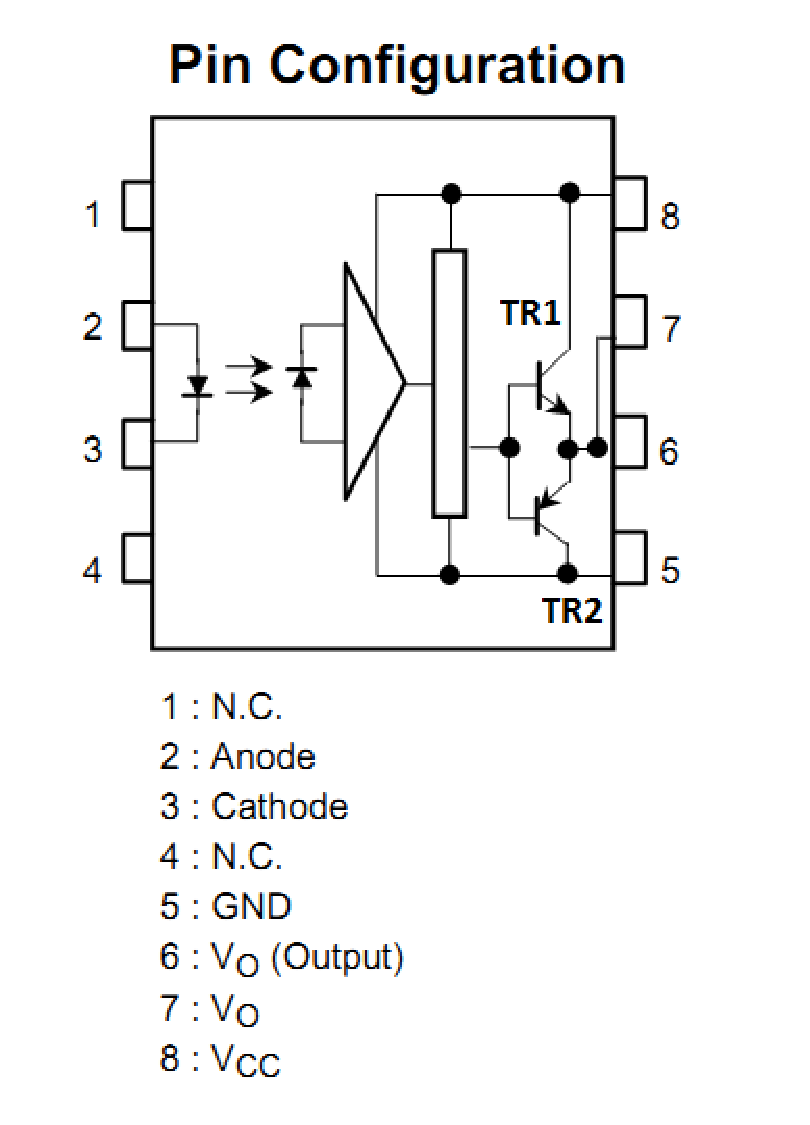
\includegraphics[width=\columnwidth]{./figs/pinout.eps}
\caption{ TLP350}  
\label{fig4}
\end{figure}

%\subsection{\textbf{Gate Driver circuit}}
%The pin description for Opto coupler(TLP350) is shown in fig \ref{fig4}
%Made connections as per the fig \ref{fig2}    
\begin{table}[!h]
\centering
\resizebox {\columnwidth} {!} {
\input{./figs/connections.tex}
}
\caption{Pin Connections} 
\label{table:connections}
\end{table}    
\begin{problem}
Program the arduino to generate a square wave with {\em Duty Cycle} $D=0.5$ and frequency $f=5KHz$.
\end{problem}
\solution
\lstinputlisting{./codes/square_wave.ino} 
\section{Fourier Series Analysis of Buck-Converter}
\begin{problem}
Observe the output of the Source pin of the n-MOS on oscilloscope and write the python script to generate the same. 
\end{problem}
\solution The output is shown in Fig. \ref{fig5}
\lstinputlisting{./codes/sqaure_wave.py} 

\begin{figure}[h]
	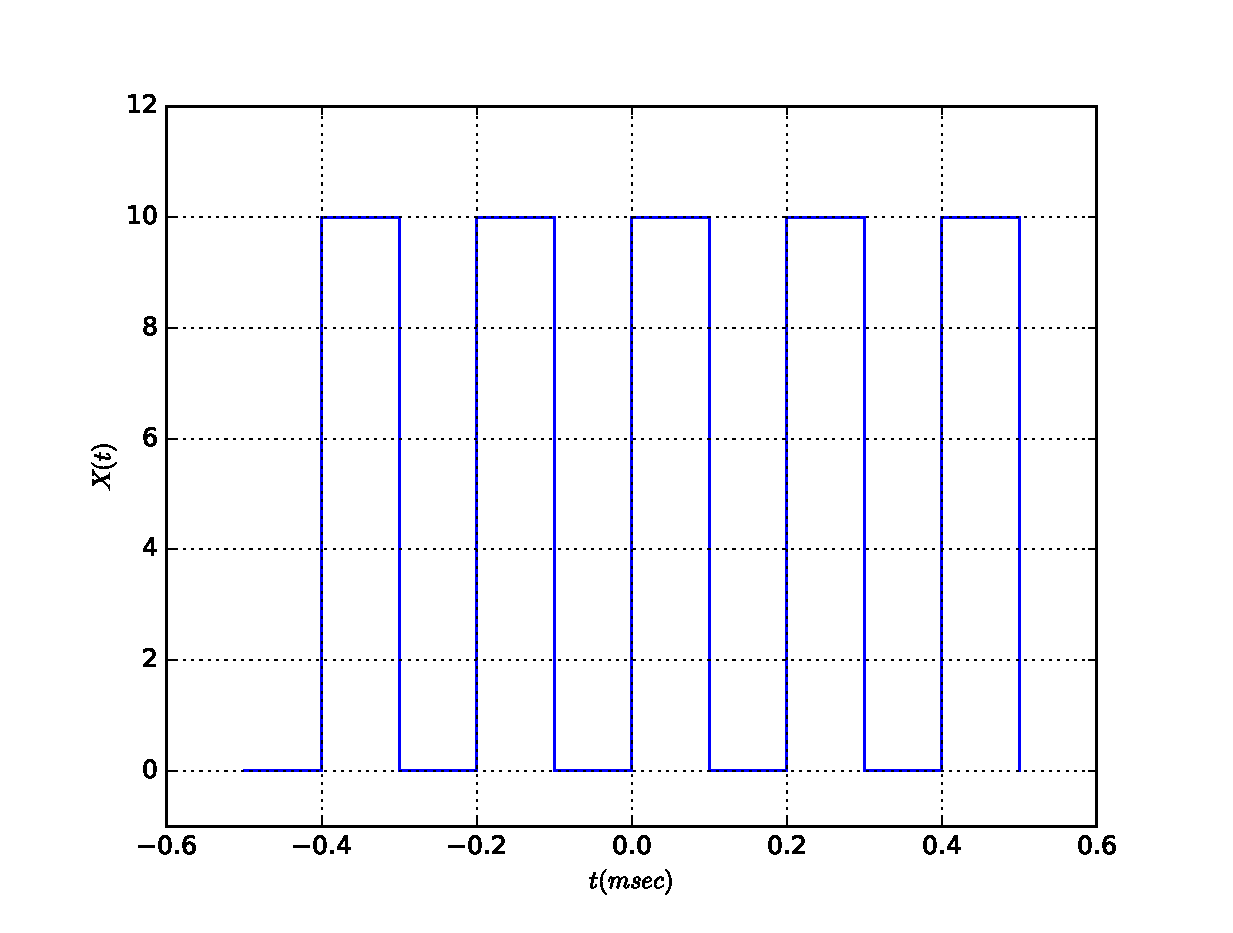
\includegraphics[scale=0.5]{./figs/square.eps}
	\caption{Square Pulse} \label{fig5}
    \end{figure}
\begin{problem}
Show that the voltage across the diode in Fig. \ref{fig1} is
%
%\begin{equation}
%X(t) = \sum_{n=0}^{\infty}a_n\cos 2\pi n f t + b_n \sin 2 \pi n f t
%\end{equation}
%is known as the Fourier series expansion of $X(t)$, where $f = \frac{1}{T}$.  Find 
%\begin{align}
%a_n &= \frac{2}{T} \int_{0}^{T}X(t) \cos 2\pi nf t \, dt \\
%b_n &= \frac{2}{T} \int_{0}^{T}X(t) \sin 2\pi nf t \, dt
%\end{align}
%Show that Fourier series expansion for $X(t)$ is
\begin{equation}
V_D(t) =
\begin{cases}
  \sum_{n=1}^{\infty} \dfrac{10}{n \pi} \sin \Big (2\pi ft \Big ) & n \text{ odd}
 \\
 5   & n = 0
 \\
 0 & n \text{ even}
 \end{cases}
\end{equation}

\end{problem}
\begin{problem}
Compute  and sketch the frequency response for the L-C-R part of Fig. \ref{fig1} shown in Fig. \ref{fig6} for $R = 5 \Omega$ and L and C calculated using  equation \eqref{eq:eq1} and  equation \eqref{eq:eq2}. What kind of filter is it?
\end{problem}
\begin{problem}
Calculate the cut-off frequency for the filter in Fig. \ref{fig6}.  
\label{prob}
\end{problem}
\begin{figure}
       \centering  
       \resizebox {\columnwidth} {!} {
\input{./figs/lpf.tex}
}
    \caption{Filter} \label{fig6}
   \end{figure}
   \begin{problem}
   Find $V_{o}$. 
   \end{problem}
 \end{document}